% Vyřadit z obsahu
\hidefromtoc

% Změna číslování kapitol, obrázků a tabulek na římské číslice
\renewcommand \thechapter{\roman{chapter}}
\renewcommand \thesection{\roman{chapter}.\roman{section}}
\renewcommand \thesubsection{\roman{chapter}.\roman{section}.\roman{subsection}}

\renewcommand{\thefigure}{\roman{chapter}.\roman{figure}}
\renewcommand{\thetable}{\roman{chapter}.\roman{table}}


\chapter{Prílohy}

\section{Dotazník OSA} \label{sec:Priloha:Dot}
V tejto časti sa nachádza dotazník, ktorý sa využíva pri vyšetrení OSA. \ref{kap:Regulace}.



\newpage
\section{Grafické prostredie} \label{sec:Priloha:HMI}
Zobrazenie grafického užívateľského rozhrania ktorý sa využíva pri vyšetrení OSA.

\begin{figure}[H]
	\centering
	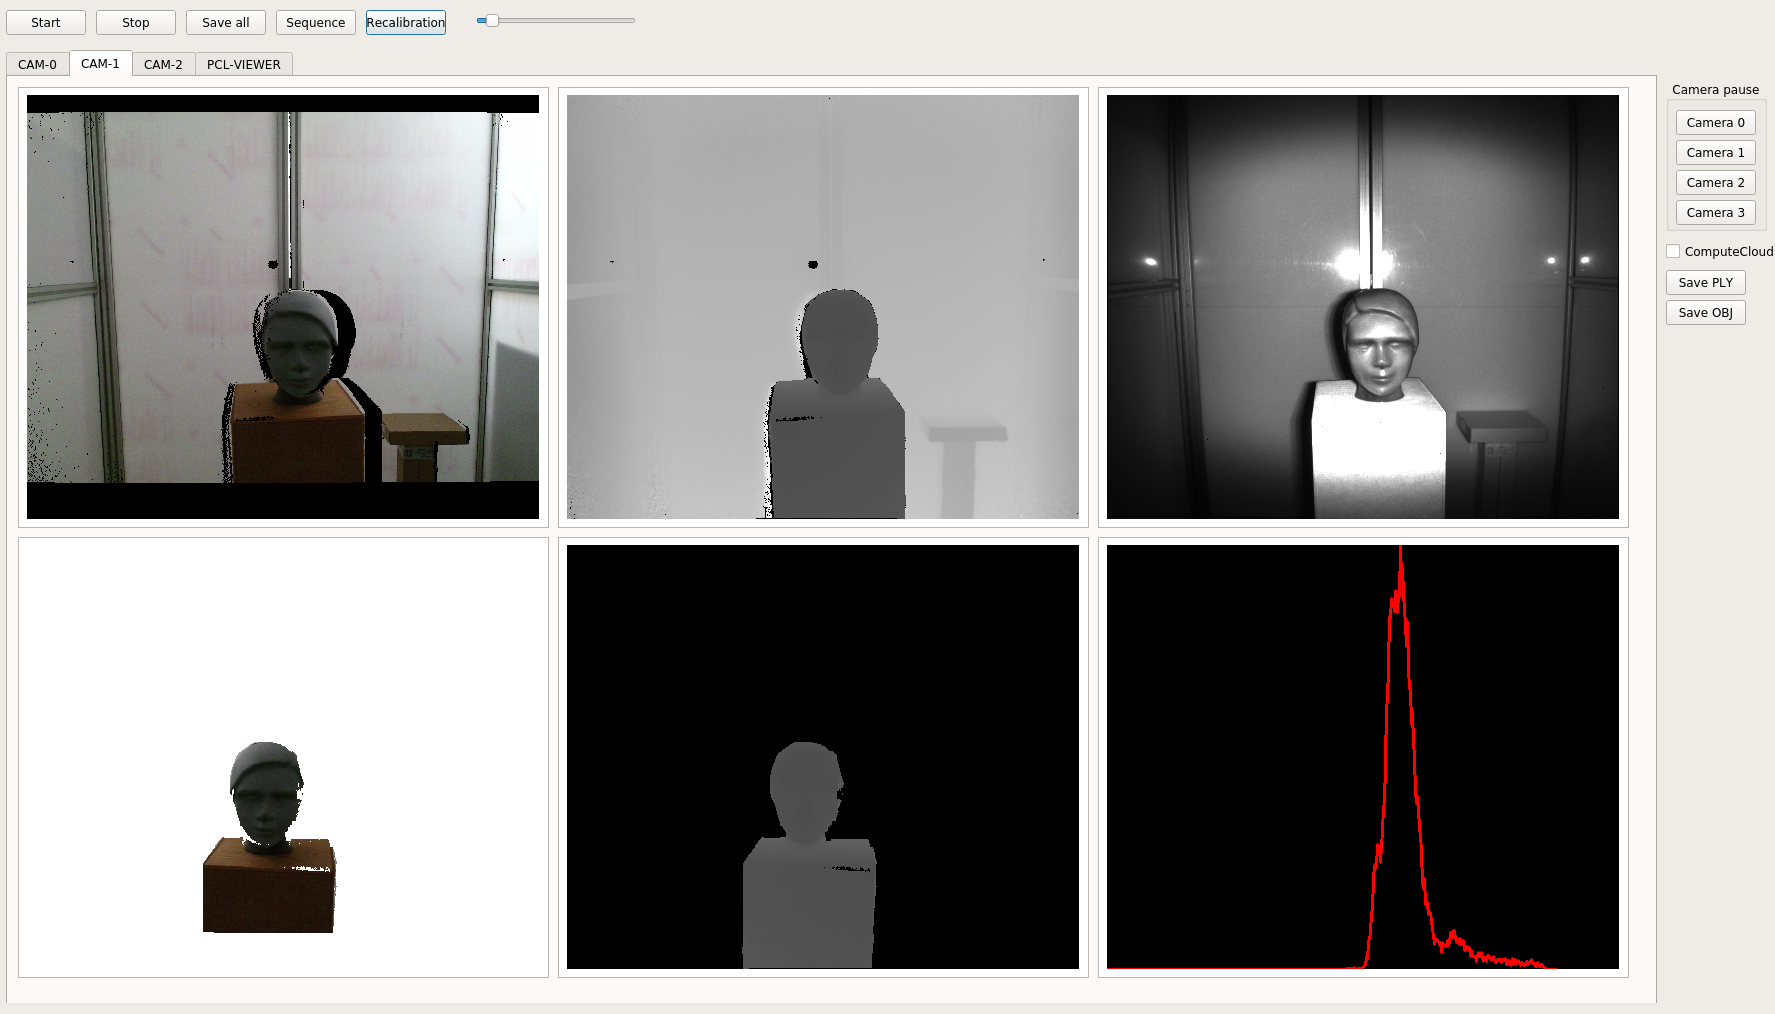
\includegraphics[width=\textwidth]{figures/hmi.png}
	\caption{Zobrazenie nadhľadov spracovávaných snímok z jednotlivých kamier.}
	\label{fig:hmi:a}
\end{figure}

\begin{figure}[H]
	\centering
	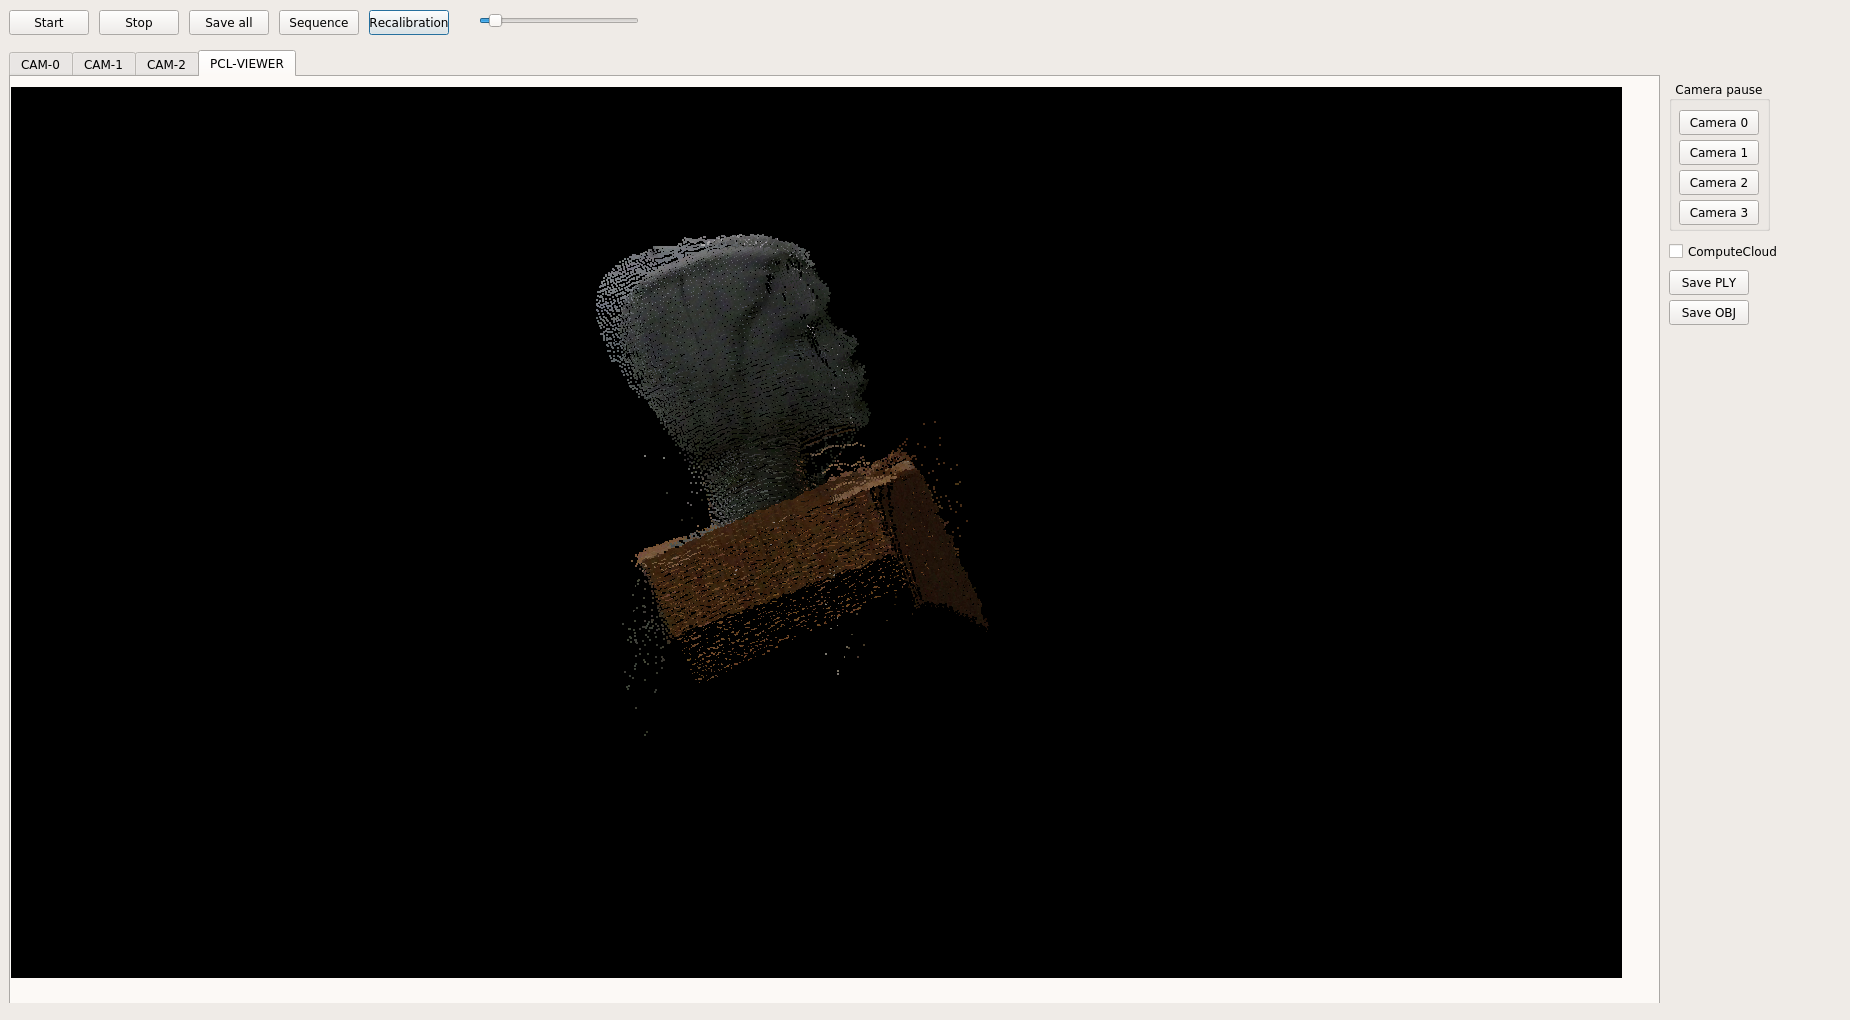
\includegraphics[width=\textwidth]{figures/hmi2.png}
	\caption{Zobrazenie mračna bodov v reálnom čase.}
	\label{fig:hmi:b}
\end{figure}

\newpage
\section{Ukážka dátového setu pre Mask R-CNN } \label{sec:Priloha:Label}

\begin{figure}[H]
	\centering
	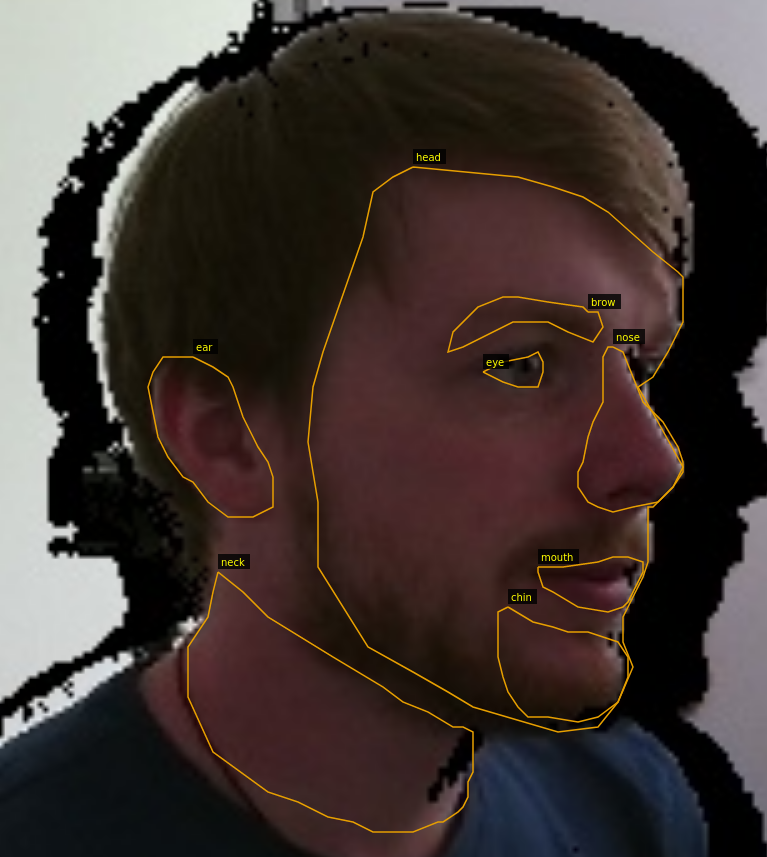
\includegraphics[width=\textwidth]{figures/rcnn_label3.png}
	\caption{RGB-D obraz použitý pri trénovaní Mask R-CNN .}
	\label{fig:mask_label}
\end{figure}

\newpage
\section{Grafické prostredie pre zber dát} \label{sec:Priloha:HMI_WEB}

\begin{figure}[H]
	\centering
	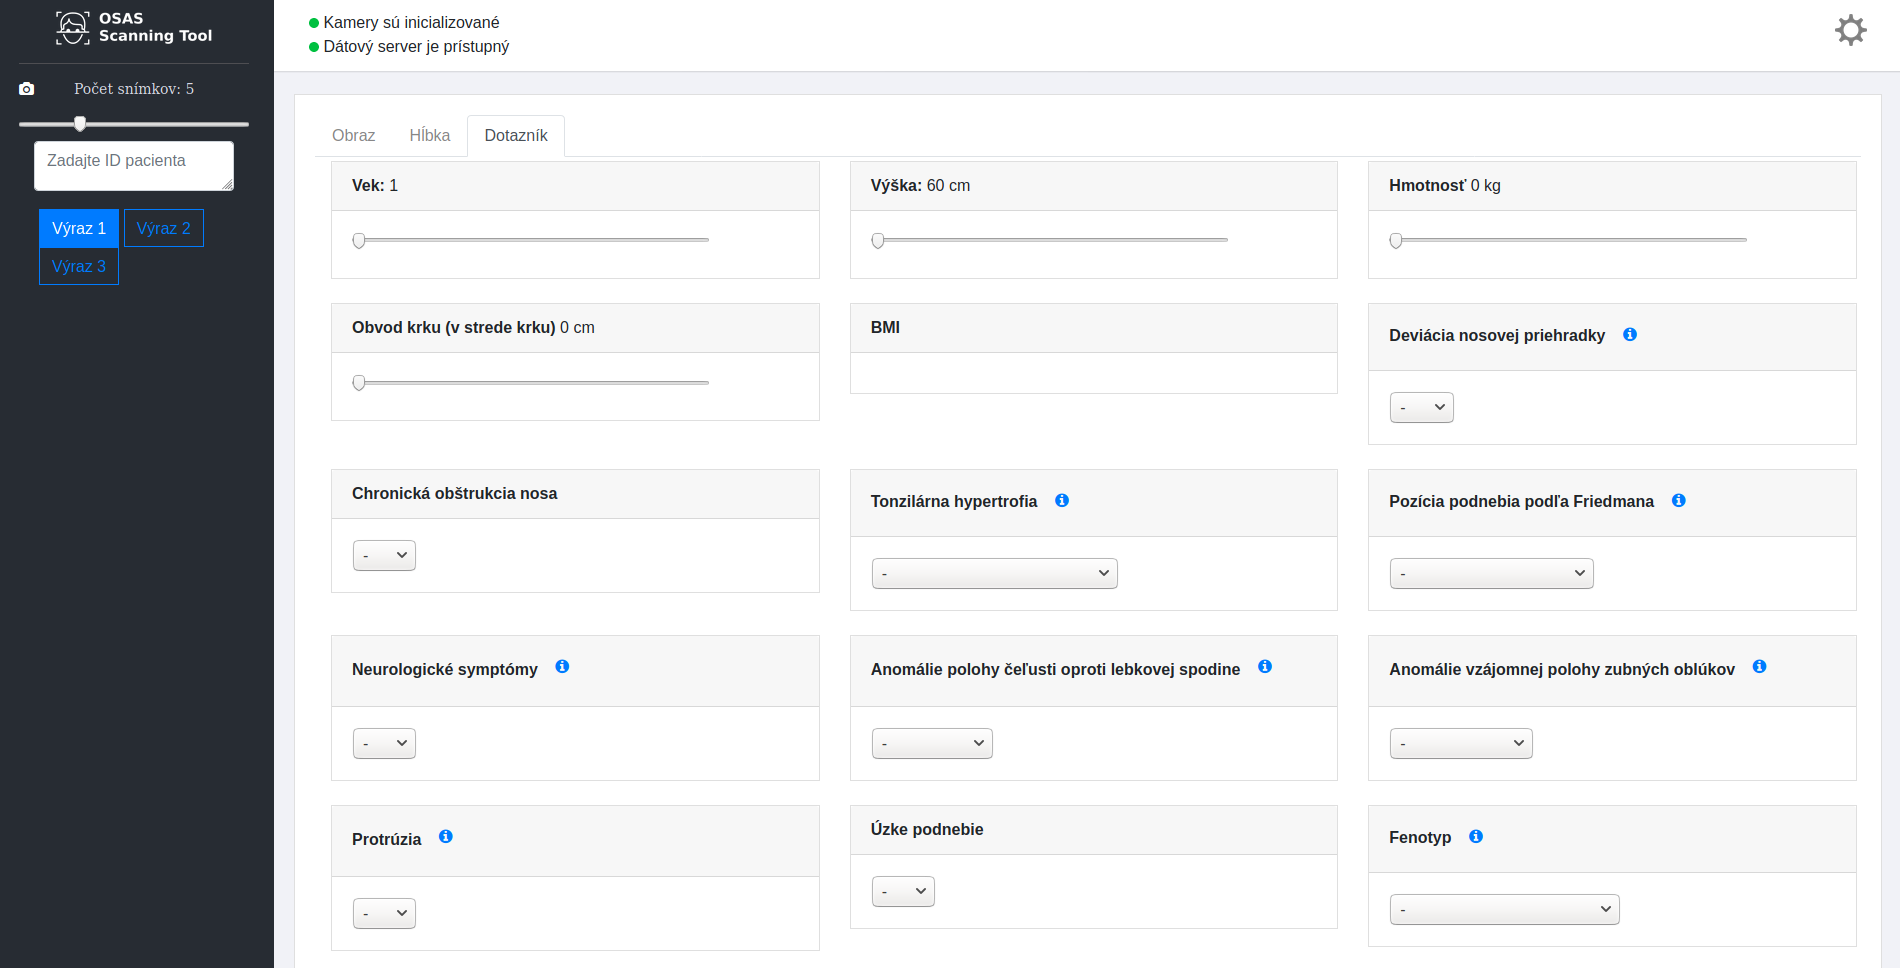
\includegraphics[width=0.85\textwidth]{figures/hmi_web3.png}
	\caption{Zobrazenie webového rozhranie pre zber dát, dotazník}
	\label{fig:hmi_web:c}
\end{figure}

\begin{figure}[H]
	\centering
	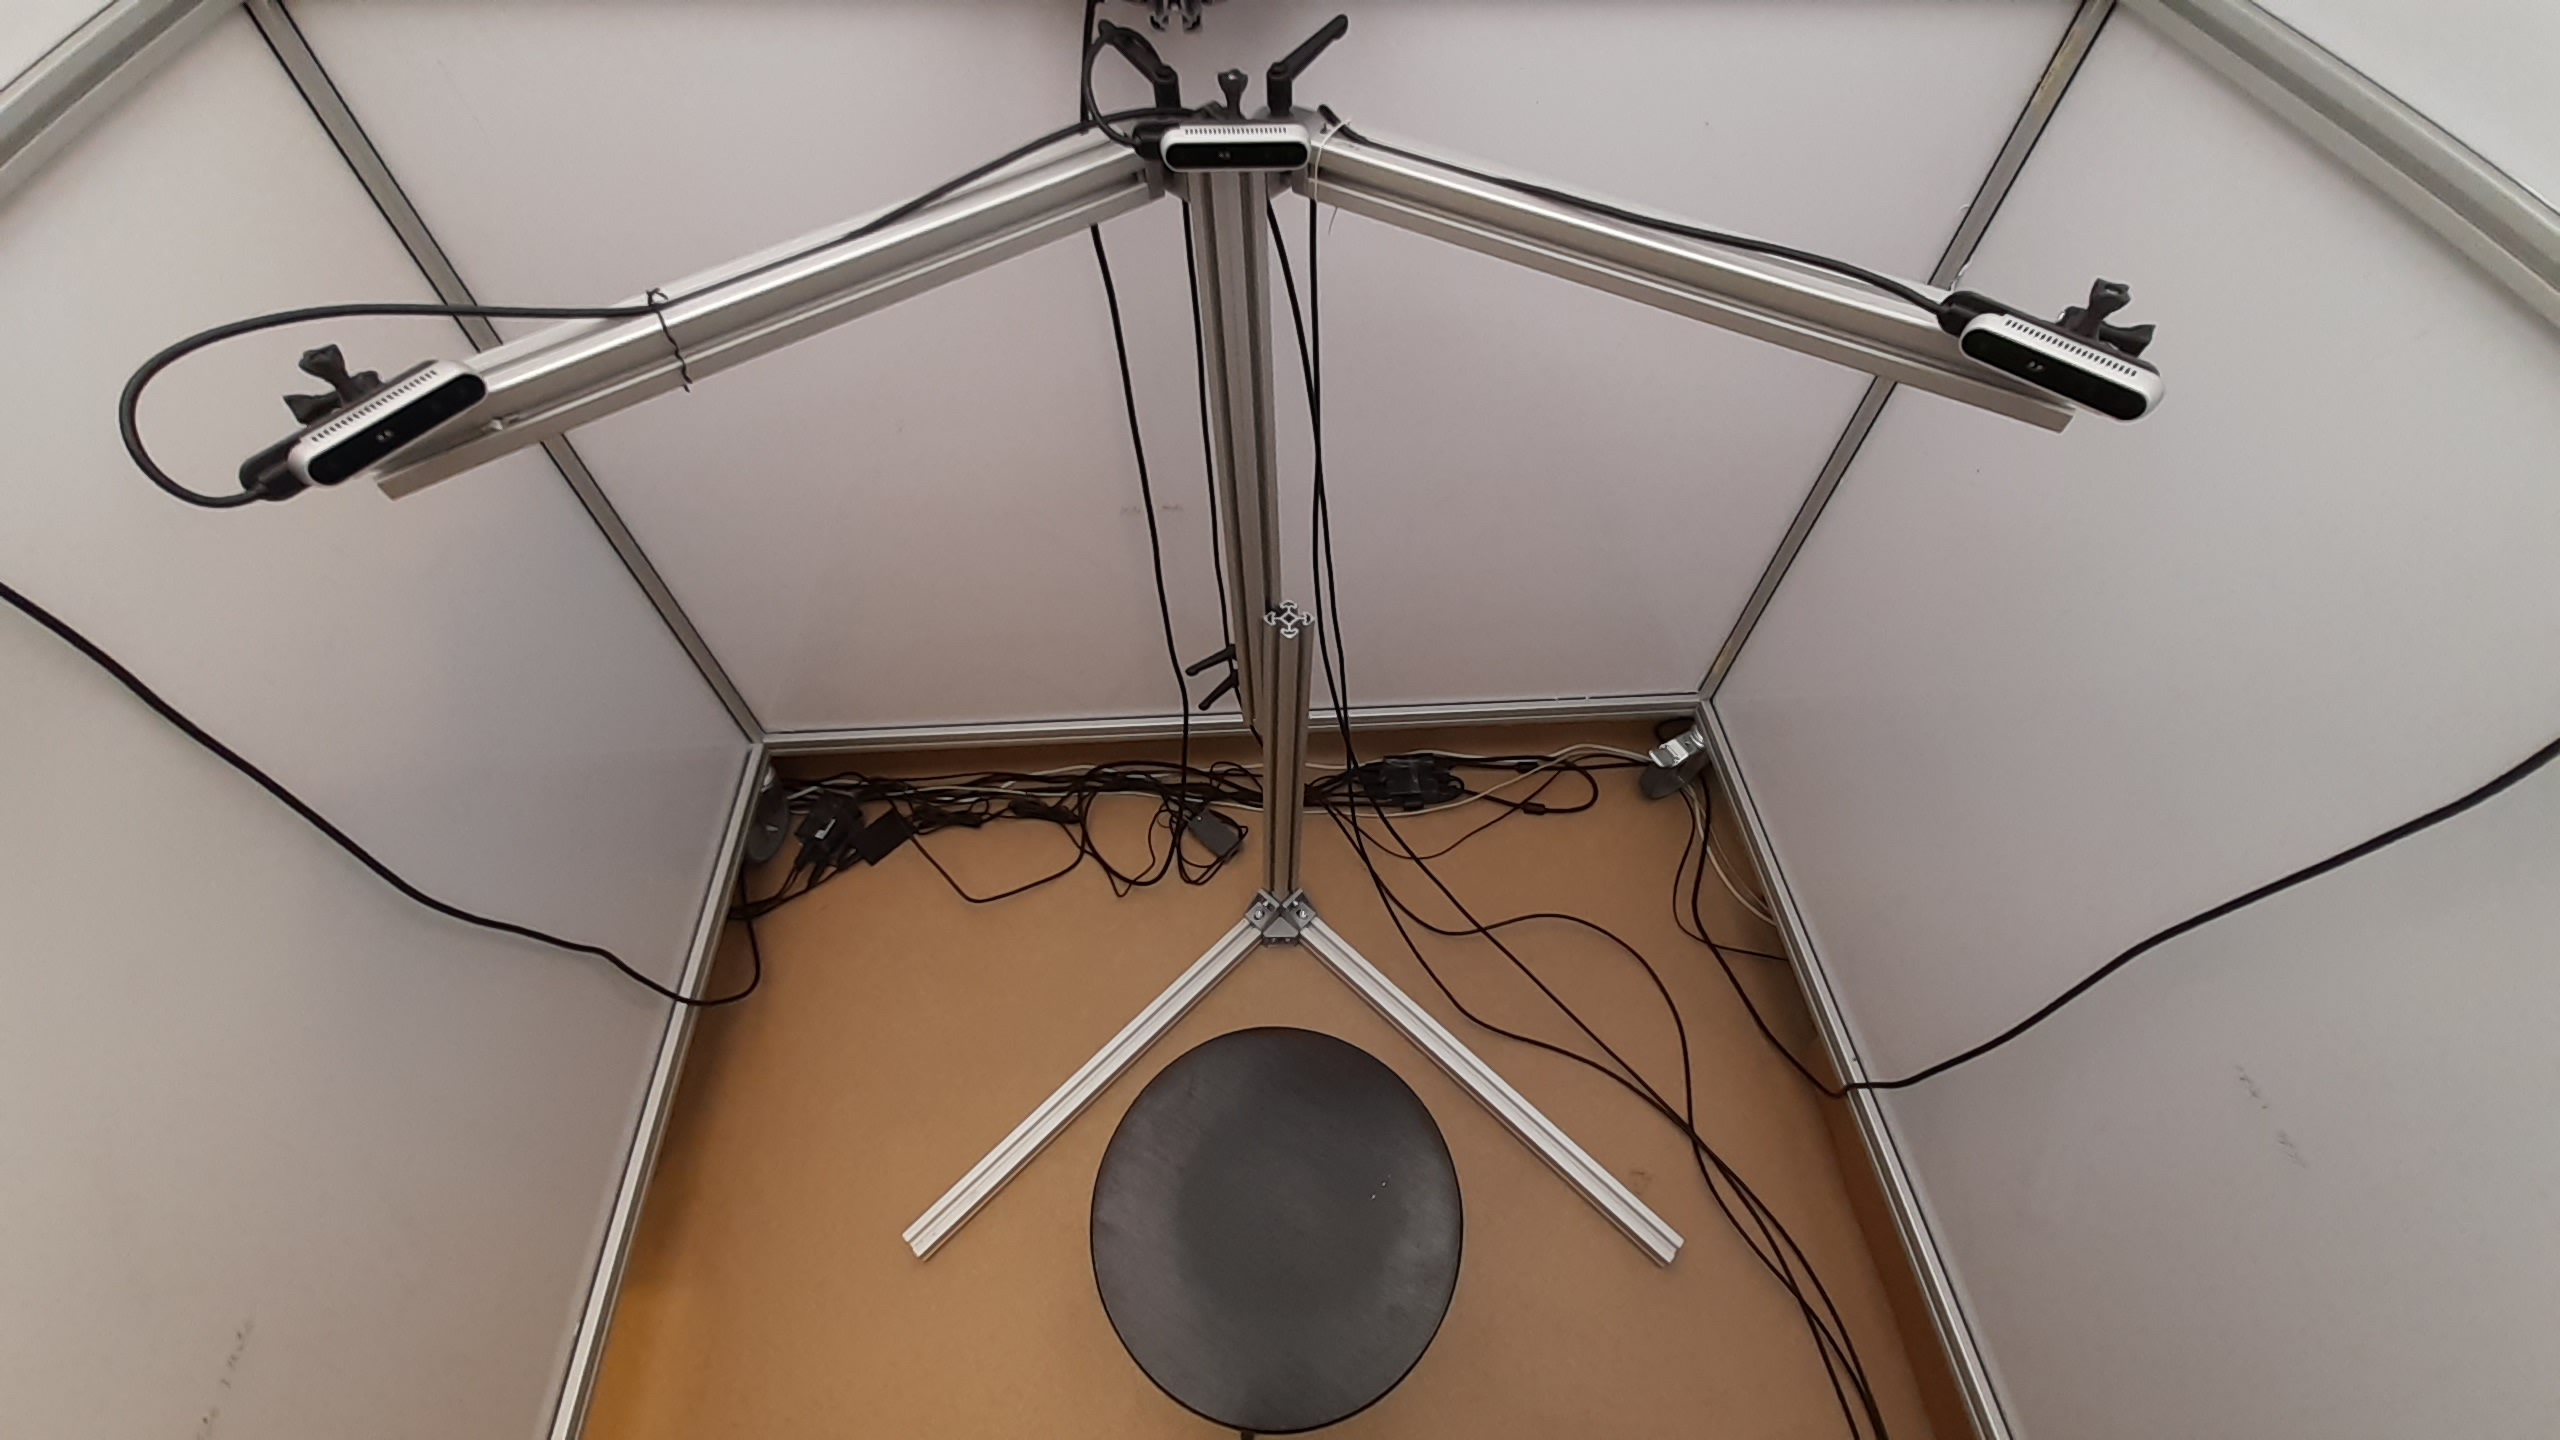
\includegraphics[width=0.85\textwidth]{figures/clinic_scaning.png}
	\caption{Konštrukcia snímacieho zariadenia použitého pre zber dát}
	\label{fig:hmi_web:d}
\end{figure}
